\documentclass[11pt]{beamer}
\usepackage[utf8]{inputenc}
\usepackage[frenchb]{babel}
\usepackage{graphicx}
\usepackage{textpos}
%%%%
%compteS

%%%
\usetheme{Berlin}
\usecolortheme{beaver}
\useinnertheme[shadow]{rounded}

\makeatletter
\beamer@theme@subsectionfalse
\makeatother

\title{UniForms}
\author[Ayoub BENATHMANE, Geneviève CIRERA, Luis Felipe POLO, Romain TRUCHI]{Ayoub BENATHMANE, Geneviève CIRERA, Luis Felipe POLO, Romain TRUCHI\\\vspace{1cm}{\small Encadrant : Michel GAUTERO}}
\institute{Polytech'Nice-Sophia}
\subtitle{Création et Partage de Formulaires 
Web et Papier}
\date{\oldstylenums{\today}}



\begin{document}
\begin{frame}
\titlepage
\end{frame}

% --------- Sommaire -----------
\begin{frame}{Plan}
  \tableofcontents[sections={1}]
  \tableofcontents[sections={2}]
  \tableofcontents[sections={3}]
  \tableofcontents[sections={4}]
\end{frame}

%\AtBeginSection[]{
%  \begin{frame}{Sommaire}
%  \small \tableofcontents[currentsection, hideothersubsections]
%  \end{frame} 
%}
% ------------------------------

% ----- Presentacion ------
\section{Introduction}
\subsection*{SubPart 1}
%\subsection{En bref}
\begin{frame}{Contexte}
	\begin{itemize}
		\item Informatisation des universités françaises
		\item Utilisation des formulaires papiers
  		\item Perte de temps
  		\item Problème de stockage
  	\end{itemize}
\end{frame}

\begin{frame}{État de l'Art}
	\begin{columns}[t]
	\begin{column}[T]{.5\textwidth}
		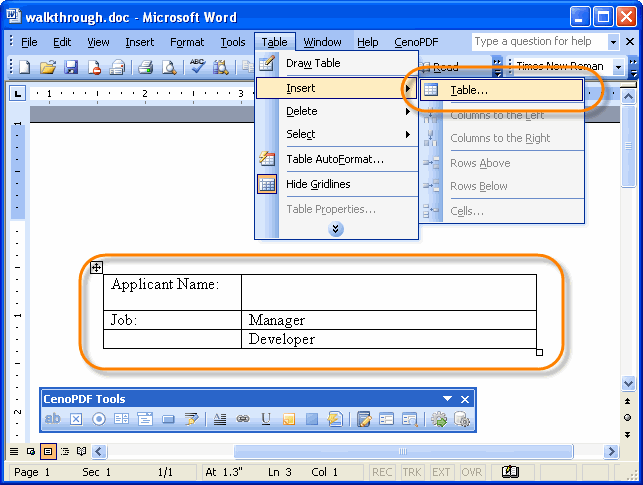
\includegraphics[width=.45\paperwidth]{images/add-table.png}
  	\end{column}
  	\begin{column}[T]{.5\textwidth}
  		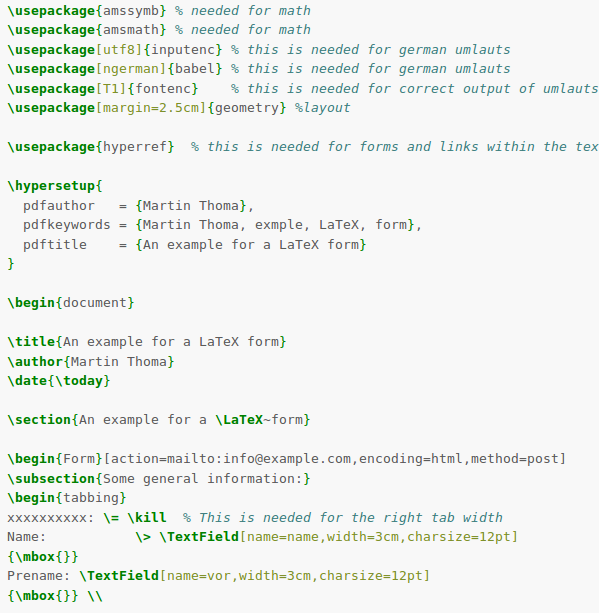
\includegraphics[width=.45\paperwidth]{images/tex.png}
	\end{column}
\end{columns}
\end{frame}
\begin{frame}{État de l'Art}
\begin{columns}[t]
	\begin{column}[T]{.5\textwidth}
		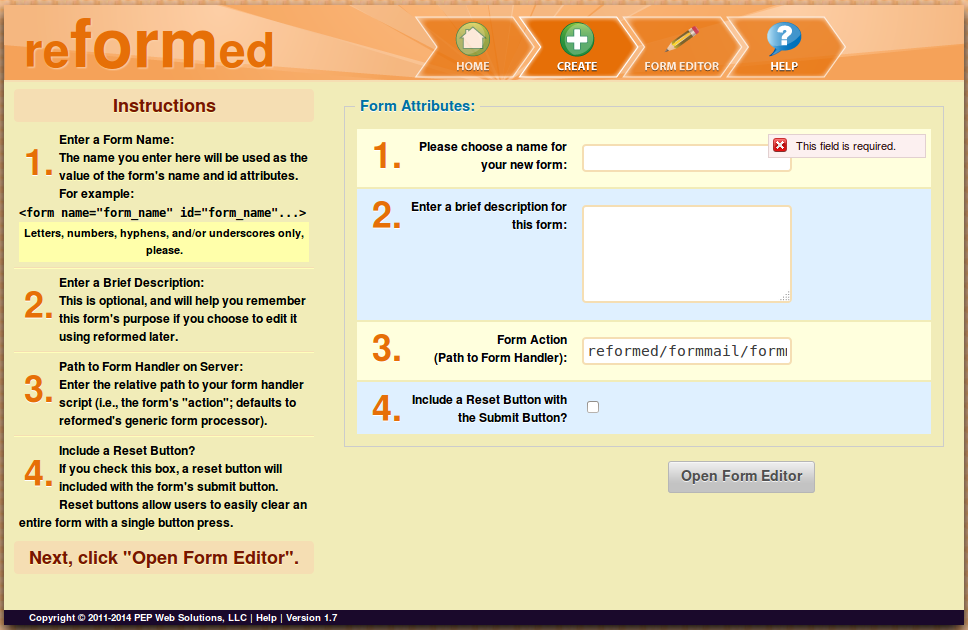
\includegraphics[width=.47\paperwidth]{images/reformed.png}
  	\end{column}
  	\begin{column}[T]{.5\textwidth}
  		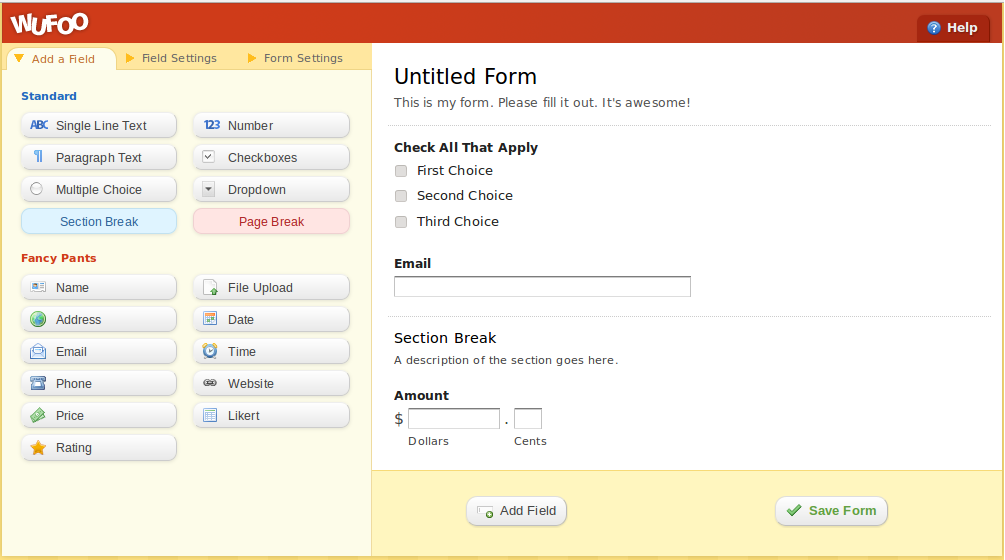
\includegraphics[width=.47\paperwidth]{images/WUFOO.png}
	\end{column}
\end{columns}
%\begin{block}{Aspects}
%	\begin{center}
%		\begin{itemize}
%			\item Utilisabilité
%			\item Nombreux éléments proposés
%			\item Anonymat
%			\item Confidentialité
%			\item Design
%   		\item Exportation
%			\item Gratuité
%	  	\end{itemize}
%	\end{center}
%\end{block}

\end{frame}

\begin{frame}{Problématiques}
\begin{block}{Comment proposer une plateforme intuitive pour la création de formulaires avec :}
	\begin{center}
		\begin{itemize}
			\item Confidentialité
			\item Collaboration
	  		\item Impression
	  		\item Accessibilité
	  	\end{itemize}
	\end{center}
\end{block}
\end{frame}






\section{Contribution}
\subsection*{SubPart 1}
\begin{frame}{Scénario : Création}
\begin{center}
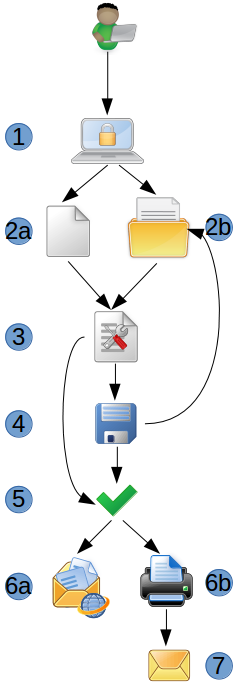
\includegraphics[width=.19\paperwidth]{images/scenario_creation.png}
\end{center}
\end{frame}

\begin{frame}{Scénarios : Répondre}
\begin{columns}[t]
	\begin{column}[T]{.5\textwidth}
		\begin{center}
		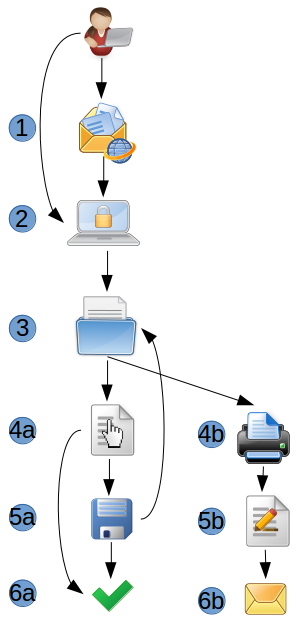
\includegraphics[width=.23\paperwidth]{images/scenario_fill.png}
		\end{center}
  	\end{column}
  	\begin{column}[T]{.5\textwidth}
  		\begin{center}
  		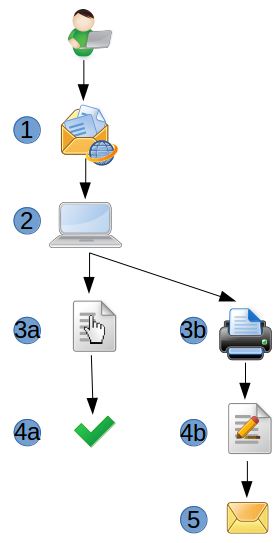
\includegraphics[width=.25\paperwidth]{images/scenario_fill_anonyme.png}
  		\end{center}
	\end{column}
\end{columns}
\end{frame}

\begin{frame}{Scénario : Exportation}
\begin{center}
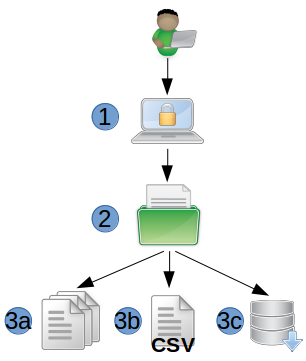
\includegraphics[width=.45\paperwidth]{images/scenario_exportation.png}
\end{center}
\end{frame}

\begin{frame}{Fonctionnalités}
\begin{itemize}
	\item Connexion CAS
	\item Questions ouvertes, fermées, mise en page 
	\item Collaboration
	\item Paramétrage des champs
	\item Ergonomie
	\item Installeur
\end{itemize}
\end{frame}

\section{Démonstration}
\subsection*{SubPart 1}
\begin{frame}{Démonstration}
\end{frame}

\section{Conclusion}
\subsection*{SubPart 1}
\begin{frame}{Conclusion}
\begin{block}{}
	\begin{center}
		Plateforme Web
	\end{center}
\end{block}
	\begin{block}{}
	\begin{center}
		Collaboration
	\end{center}
\end{block}
\begin{block}{}
	\begin{center}
		Package + Installeur
	\end{center}
\end{block}
\begin{block}{}
	\begin{center}
		Mise en page
	\end{center}
\end{block}
\end{frame}

\begin{frame}{Perspectives}
\begin{block}{}
	\begin{center}
		Création de comptes
	\end{center}
\end{block}

\begin{block}{}
	\begin{center}
		Proposer plus d'éléments
	\end{center}
\end{block}

\begin{block}{}
	\begin{center}
		Bases de données externes
	\end{center}
\end{block}
\end{frame}

\begin{frame}{}
\begin{center}
Merci de votre attention
\end{center}
\end{frame}
\end{document}